%------------------------------------------------
\section{Public health policy-making problem}
%------------------------------------------------
\begin{frame}[t,label=abm_3]
	\frametitle{Public health policy-making problem formulation}
	\tikzstyle{background grid}=[draw, black!50,step=.5cm]
	%
	What is the \emphasis{cost} of public health interventions?\\
	%
	\begin{columns}[t] % The "c" option specifies centered vertical alignment while the "t" option is used for top vertical alignment
		\begin{column}{.5\textwidth} % Left column and width

			\begin{tikzpicture}[remember picture, overlay] %show background grid, 
				\node [inner sep=0pt,above right, opacity=1.0]  at (0.0\textwidth,-0.66\textheight) (abm) 
					{
						\only<-5>{
							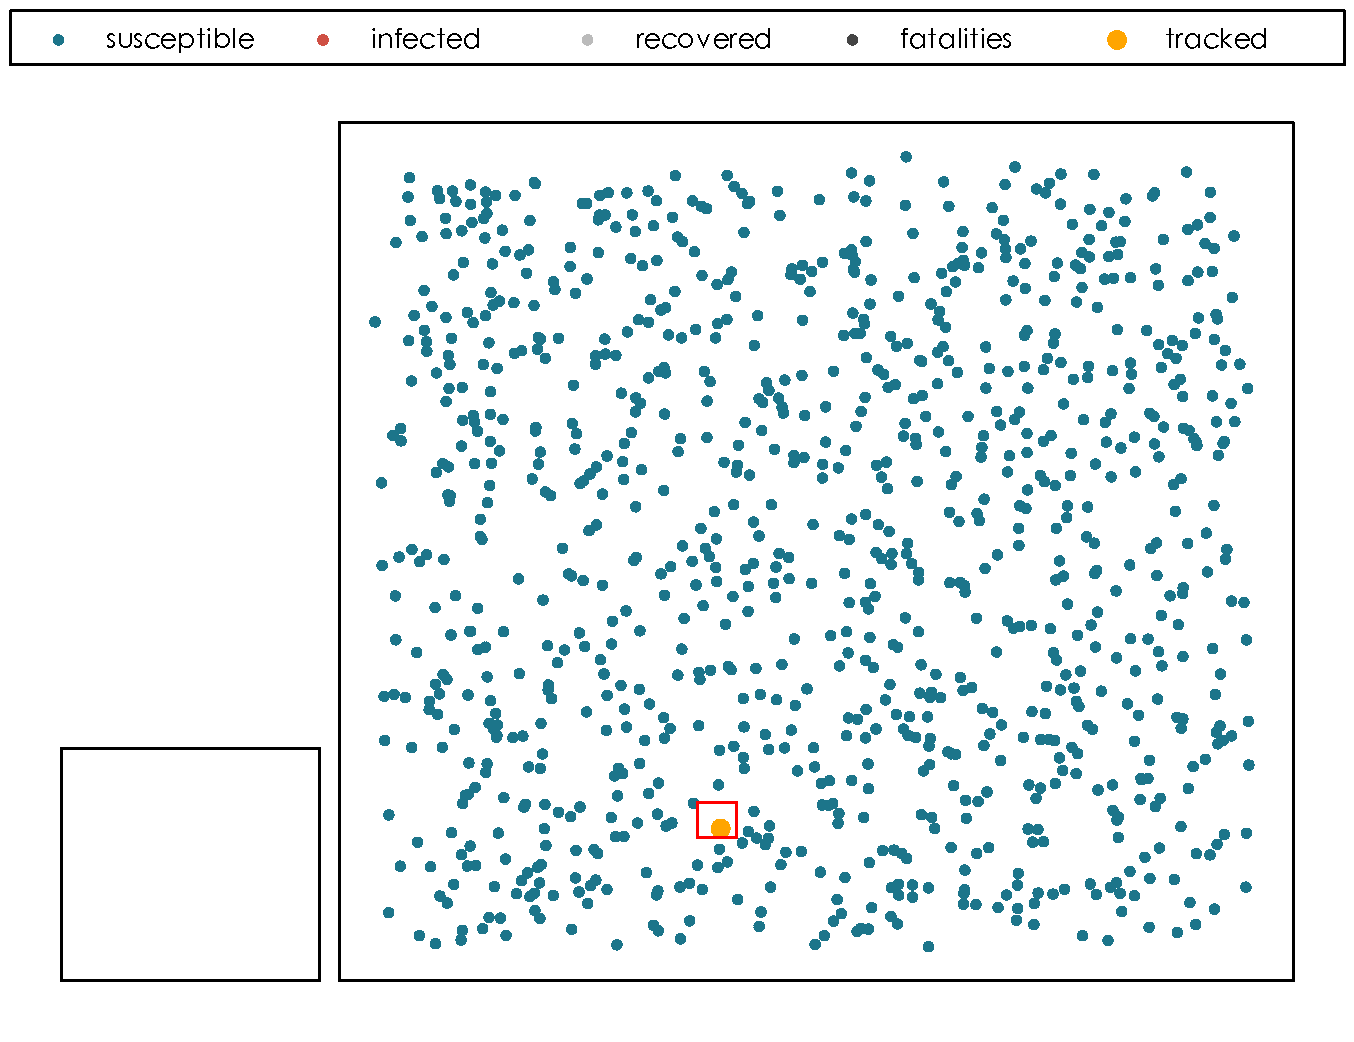
\includegraphics[width=0.95\textwidth]{render_2_no_restrictions/sim_10.pdf}
						}%	
						\only<6>{
							\begin{animateinline}[autoplay,width=0.95\textwidth]{70}
								\ifshowanimations
									\multiframe{77}{i=10+45}{%
										\includegraphics{render_2_no_restrictions/sim_\i.pdf}
									}
								\else
									\multiframe{1}{i=10+0}{%
										\includegraphics{render_2_no_restrictions/sim_\i.pdf}
									}
								\fi
							\end{animateinline}%
						}%
						\only<7>{
							\includegraphics[width=0.95\textwidth]{render_2_no_restrictions/sim_3500.pdf}
						}%
					};
				\only<1-7>{\node[inner sep=0pt,align=flush center,above=\belowcaptionskip of abm,text width=\linewidth]
					{\vspace{-1em}{\large No interventions applied}};}%
				%
				\node [inner sep=0pt,above right, opacity=1.0]  at (0.0\textwidth,-0.69\textheight) (infection) 
				{
					\only<8>{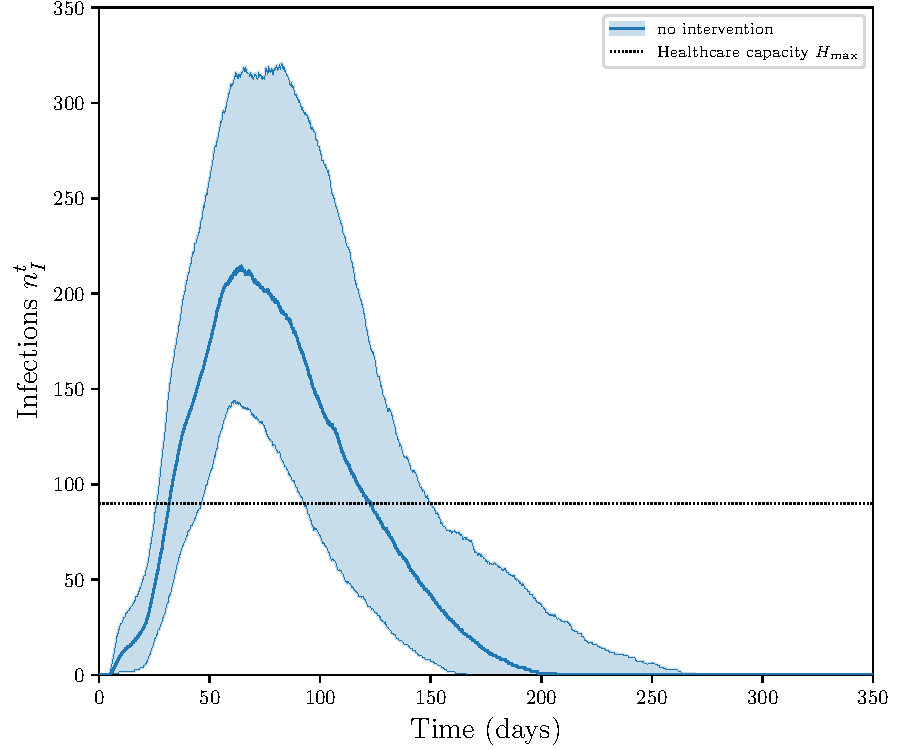
\includegraphics[width=0.9\textwidth]{trajectory_demo/I_compare_opt_1.pdf}}%
					\only<9>{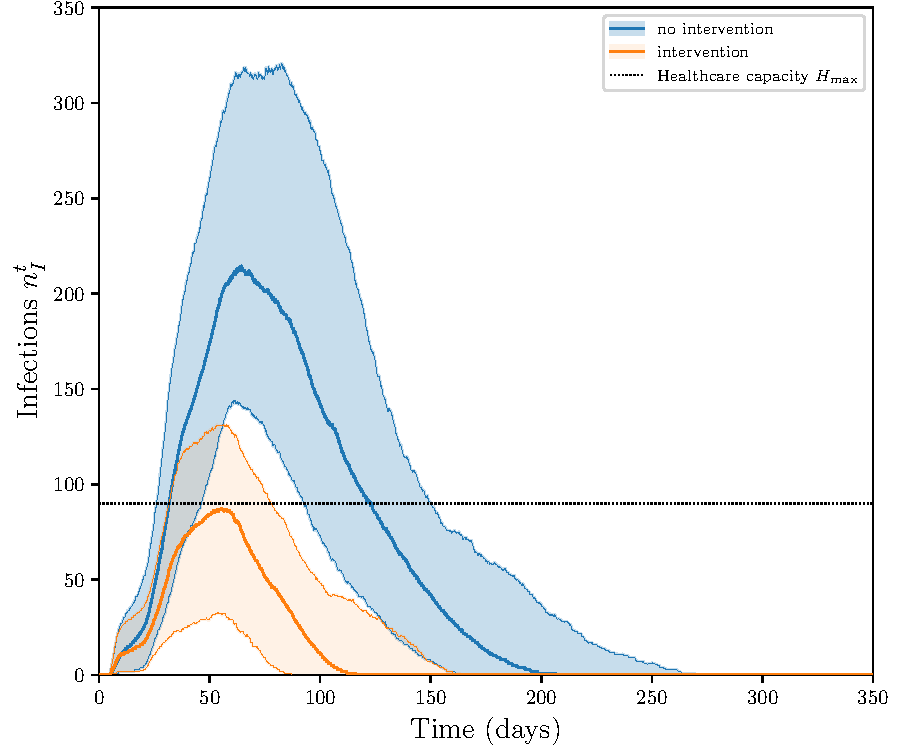
\includegraphics[width=0.9\textwidth]{trajectory_demo/I_compare_opt_3.pdf}}%
				};

				\only<9>{
					\node[inner sep=0pt,align=flush center,above=\belowcaptionskip of infection,text width=\linewidth]
					{\vspace{-1em}{
						\large {\color{darkgreen} infections $\downarrow$}
					}};
				}%

			\end{tikzpicture}%

		\end{column}
		%
		\begin{column}{.5\textwidth} % Left column and width

			\tikzstyle{background grid}=[draw, black!50,step=.1cm]
			\begin{tikzpicture}[remember picture, overlay] %show background grid, 
				\node [inner sep=0pt,above right, opacity=1.0]  at (0.0\textwidth,-0.66\textheight) (abm) 
					{
						\only<2-5>{
							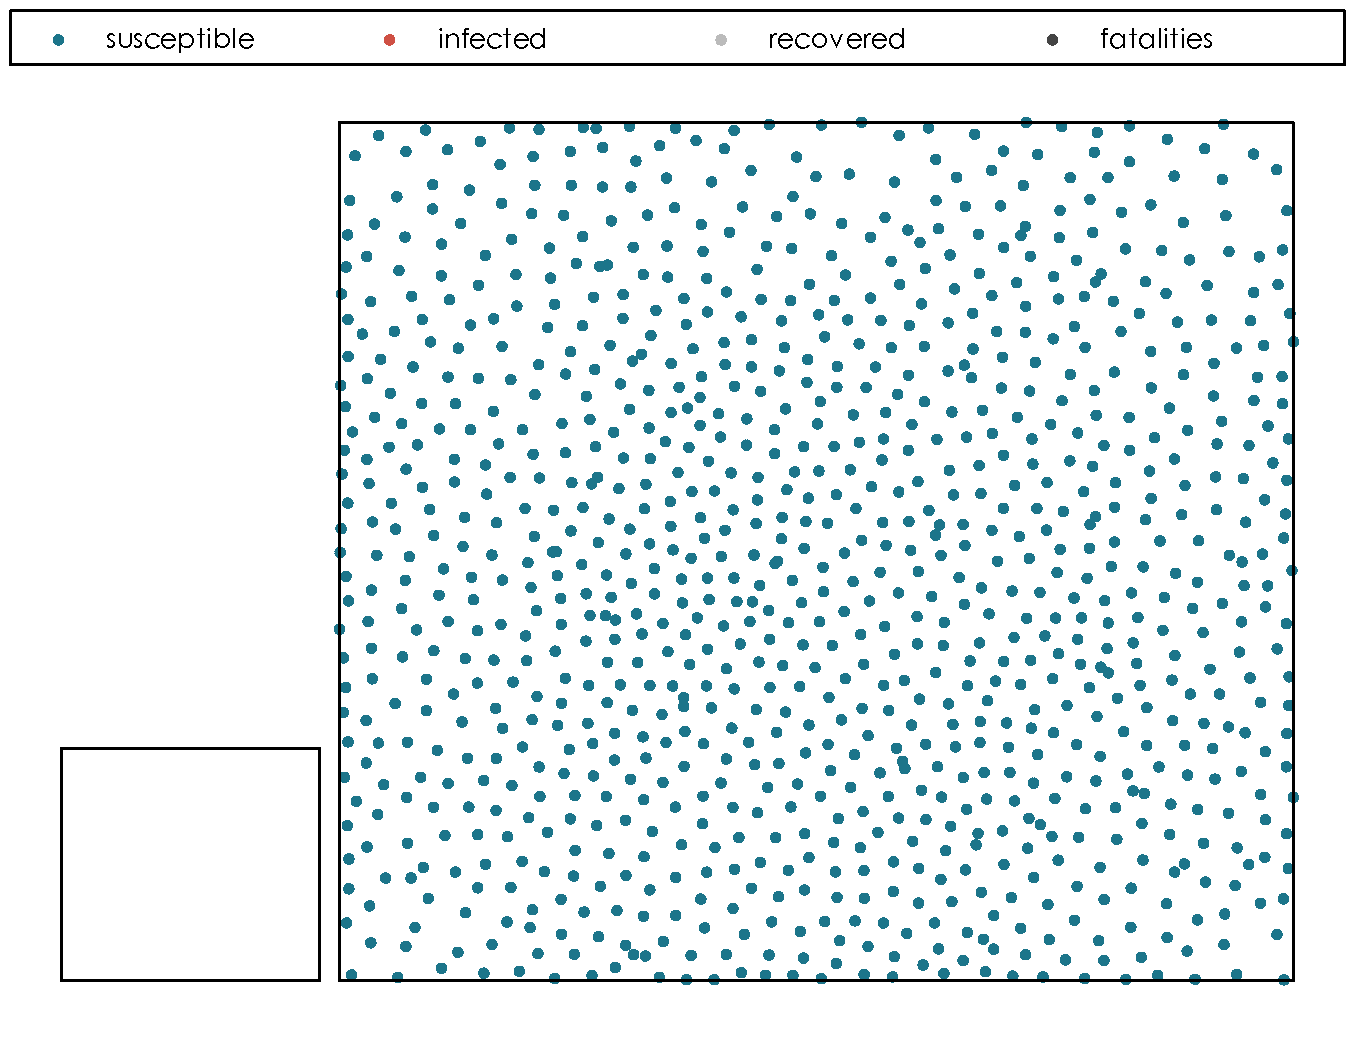
\includegraphics[width=0.95\textwidth]{render_1_restrictions/sim_50.pdf}
						}%	
						\only<6>{
							\begin{animateinline}[autoplay,width=0.95\textwidth]{70}
								\ifshowanimations
									\multiframe{75}{i=50+45}{%
										\includegraphics{render_1_restrictions/sim_\i.pdf}
									}
								\else
									\multiframe{1}{i=50+0}{%
										\includegraphics{render_1_restrictions/sim_\i.pdf}
									}
								\fi
							\end{animateinline}%
						}%
						\only<7>{
							\includegraphics[width=0.95\textwidth]{render_1_restrictions/sim_3500.pdf}
						}%
					};
				\only<3-7>{\node[inner sep=0pt,align=flush center,above=\belowcaptionskip of abm,text width=\linewidth]
					{\vspace{-1em}{\large with intervention}};}%
				%
				\node [inner sep=0pt,above right, opacity=1.0]  at (0.0\textwidth,-0.69\textheight) (mobility) 
				{
					\only<8>{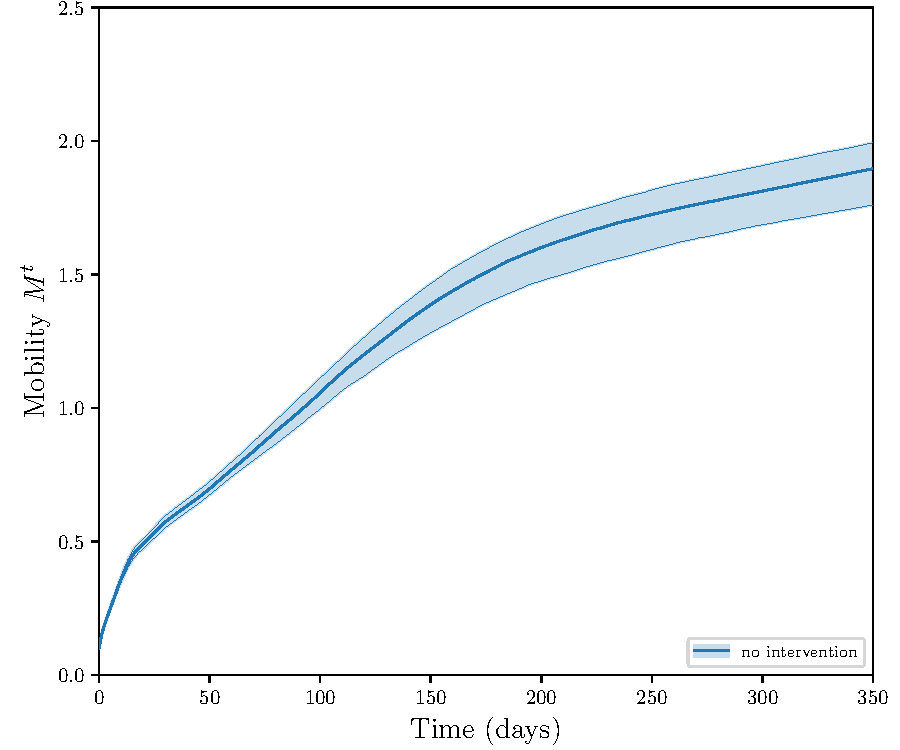
\includegraphics[width=0.9\textwidth]{trajectory_demo/M_compare_opt_1.pdf}}%
					\only<9>{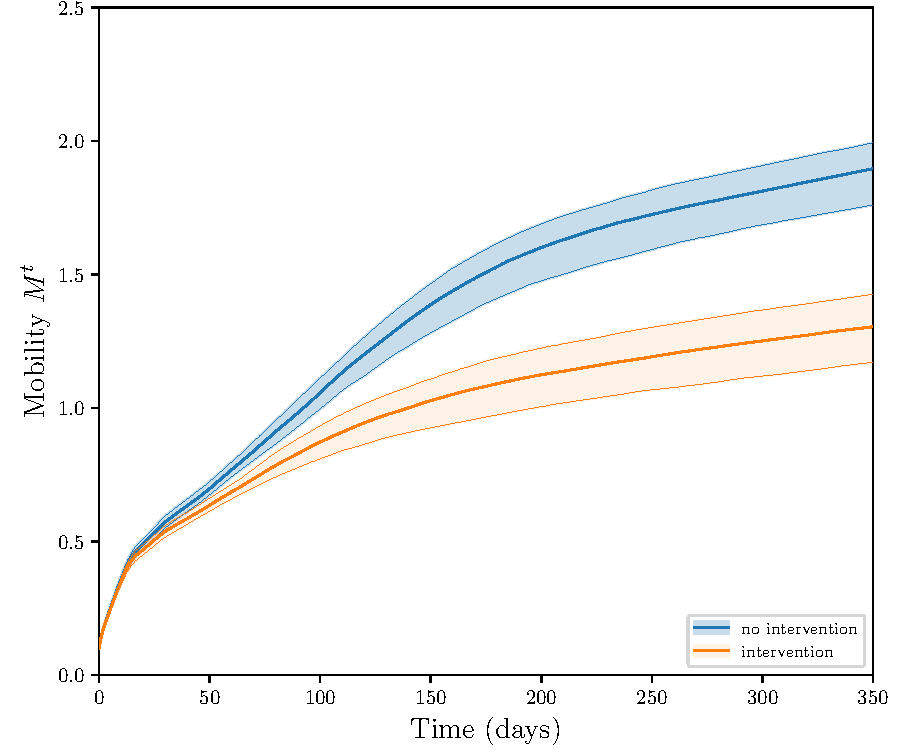
\includegraphics[width=0.9\textwidth]{trajectory_demo/M_compare_opt_3.pdf}}%
				};
				\only<3>{
					\node [draw=black, line width=0.1mm, fill=white, inner sep=5pt,above right, opacity=1.0]  at (0.5,-1.5) (text eworker) 
						{
							\Large essential workers
						};
					\node [above right] at (3,-3.5) (eworker) {};
					\draw[-stealth,line width=2pt] (text eworker.south) to [in=90,out=270] (eworker);
				}%
				\only<4>{
					\node [draw=black, line width=0.1mm, fill=white, inner sep=5pt,above right, opacity=1.0]  at (0.5,-1.5) (text hospital) 
						{
							\Large testing and quarantine
						};
					\node [above right] at (1,-4.5) (hospital) {};
					\draw[-stealth,line width=2pt] (text hospital.south) to [in=90,out=270] (hospital);
				}%
				\only<5>{
					\node [draw=black, line width=0.1mm, fill=white, inner sep=5pt,above right, opacity=1.0]  at (0.5,-1.5) (text sd) 
						{
							\Large social distancing
						};
					\node [above right] at (2.6,-4.7) (sd) {};
					\node [above right] at (2.2,-5.5) (a1) {};
					\node [above right] at (2.7,-4.5) (a2) {};
					\draw[-stealth,line width=2pt] (text sd.south) to [in=90,out=270] (sd);
					\draw[stealth-stealth,line width=2pt,red] (a1) to (a2);
				}%
				\only<9->{
					\node[inner sep=0pt,align=flush center,above=\belowcaptionskip of mobility,text width=\linewidth]
					{\vspace{-1em}{
						\large {\color{red} mobility $\downarrow$}
					}};
				}%
				% show origin
				% \fill (0,0) circle (2pt);
			\end{tikzpicture}%
		\end{column}

	\end{columns}
	\vspace{-3em}
\end{frame}
%------------------------------------------------
\begin{frame}[t,label=abm_4]
	\frametitle{Optimization problem}
	\tikzstyle{background grid}=[draw, black!50,step=.5cm]
	%
	\uncover<2->{No gradient information available, blackbox is expensive and \only<3->{\emphasis}{noisy}}\\
	%
	\begin{columns}[t] % The "c" option specifies centered vertical alignment while the "t" option is used for top vertical alignment
		\begin{column}{.42\textwidth} % Left column and width
			\vspace{-1.2em}
			% Optimization problem
			\begin{exampleblock}{Objective and constraints}
				\only<1-3>{
					\begin{equation*}
						\begin{aligned}
							& \underset{\mathbf{x}}{\text{min}}
							& & f(\mathbf{x}) = -M^{T}\\
							& \text{subject to}
							& & \uncover<2->{{c}(\mathbf{x}) \equiv n_{I,\text{max}} - H_{\text{max}} \le 0}\\
							& \text{where}
							& & \mathbf{x}=\left[n_E,S_D,n_T\right]^\mathit{T}\\
						\end{aligned}
					\end{equation*}
				}%
				\only<4->{
					\vspace{-1.2em}
					\begin{equation*}
						\begin{aligned}
							& \underset{\mathbf{x}}{\text{min}}
							& & f(\mathbf{x}) = \mathbb{E}_{\Theta}\left[{f}_{\Theta}(\mathbf{x}) = -M^{T}\right]\\
							& \text{subject to}
							& & {c}(\mathbf{x}) = \mathbb{E}_{\Theta}\left[{c}_{\Theta}(\mathbf{x}) \equiv n_{I,\text{max}} - H_{\text{max}}\right] \le 0\\
							& \text{where}
							& & \mathbf{x}=\left[n_E,S_D,n_T\right]^\mathit{T},{\color{red}\Theta\mathrm{:realizations}}
						\end{aligned}
					\end{equation*}
				}%
			\end{exampleblock}
			\vspace{-0.5em}
			\uncover<1->{
				% Variables
				\begin{alertblock}{Design variables}
					\vspace{-0.0em}
						\begin{itemize}\itemsep0em
							\item $n_E:$ Number of essential workers
							\item $S_D:$ Social distancing factor
							\item $n_T:$ Number of tests daily
						\end{itemize}
				\end{alertblock}
			}%
			\vspace{-0.5em}
			\uncover<5->{
				% Parameters
				\begin{blueblock}{Randomly seeded parameters}
					\vspace{-0.0em}
					\begin{itemize}\itemsep0em
						\item Initial conditions
						\item Interactions, demographics
					\end{itemize}
				\end{blueblock}
			}%
		\end{column}
		%
		\begin{column}{.5\textwidth} % Left column and width
			\tikzstyle{background grid}=[draw, black!50,step=.5cm]
			\begin{tikzpicture}[remember picture, overlay]%[show background grid]
				\only<1-5>{
					\node [inner sep=0pt,above right, opacity=1.0] at (0, -4.5) (objective)
						{
							\only<1->{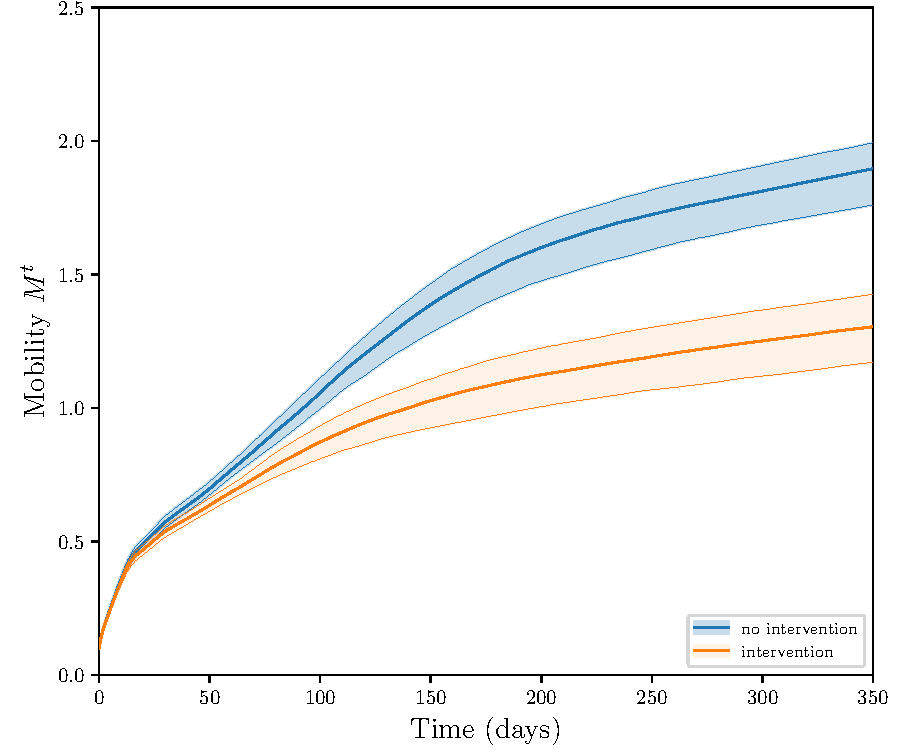
\includegraphics[width=0.7\textwidth]{trajectory_demo/M_compare_opt_3.pdf}}%
						};
					\only<1->{
						\node [above right] at (3.2,-3.5) (a1) {};
						\node [above right] at (2.2,-1.5) (a2) {};
						\draw[-stealth,line width=2pt,black] (a1) to [out=90, in=310] (a2);
					}
					\node [inner sep=0pt,above right, opacity=0.7] at (2.5, -6.5) (constraint)
						{
							\only<2->{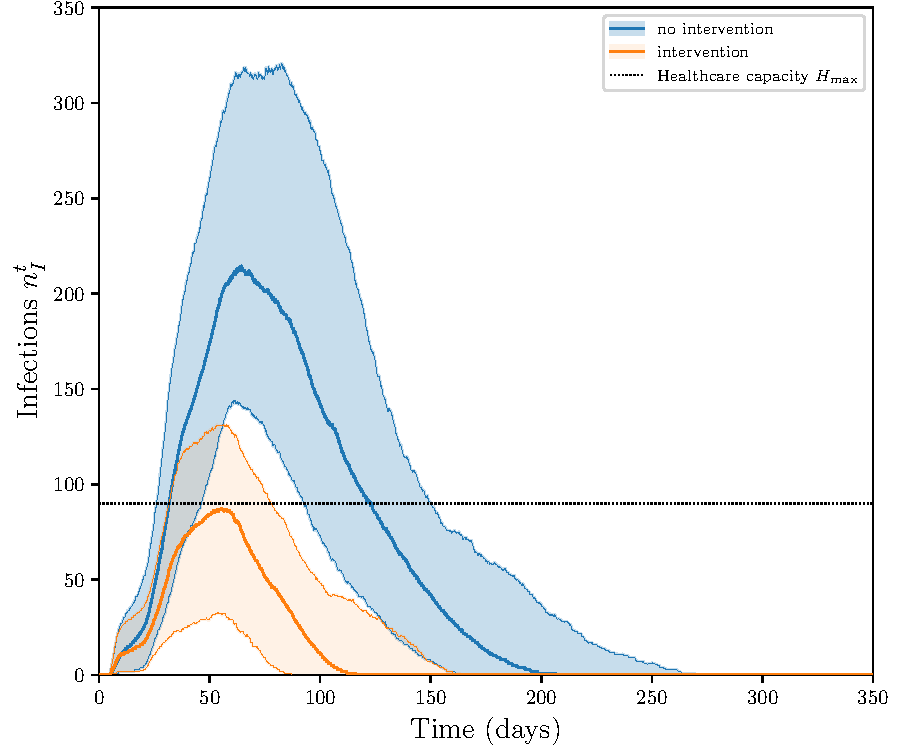
\includegraphics[width=0.7\textwidth]{trajectory_demo/I_compare_opt_3.pdf}}%
						};
					\only<2->{
						\node [above right] at (4.7,-3.5) (a1) {};
						\node [above right] at (3.7,-5.5) (a2) {};
						\draw[-stealth,line width=2pt,black] (a1) to [out=210, in=90] (a2);
					}					

				}%
				% show origin
				% \fill (0,0) circle (2pt);
				% define destination coordinates
			\end{tikzpicture}%
		\end{column}
	
	\end{columns}
	\vspace{-3em}
\end{frame}